\documentclass[xetex,table]{beamer}

\usepackage{fontspec}
\usepackage[autostyle]{csquotes}
\usepackage{hyperref}
\usepackage{color}
\usepackage{setspace}
\usepackage{listings}

\usetheme{Pittsburgh}
\usecolortheme{beaver}

\title{Linux e Circuiti elettronici}
\subtitle{con Scratch e Raspberry Pi}
\author{Luca Ceresoli}
\date{}

\AtBeginSection[]{
  \begin{frame}{}
    \huge
    \begin{center}
      \insertsection
    \end{center}
  \end{frame}
}

\begin{document}

\maketitle

\section{Circuiti elettrici}

\begin{frame}
  \frametitle{Circuiti idraulici}
  \begin{center}
    \includegraphics[height=0.6\textheight]{images/hydraulic-circuit.pdf}
  \end{center}
\end{frame}

\begin{frame}
  \frametitle{Circuiti elettrici}
  \begin{center}
    \includegraphics[height=0.6\textheight]{images/led-circuit.pdf}
  \end{center}
\end{frame}

\begin{frame}
  \frametitle{Un diodo LED}
  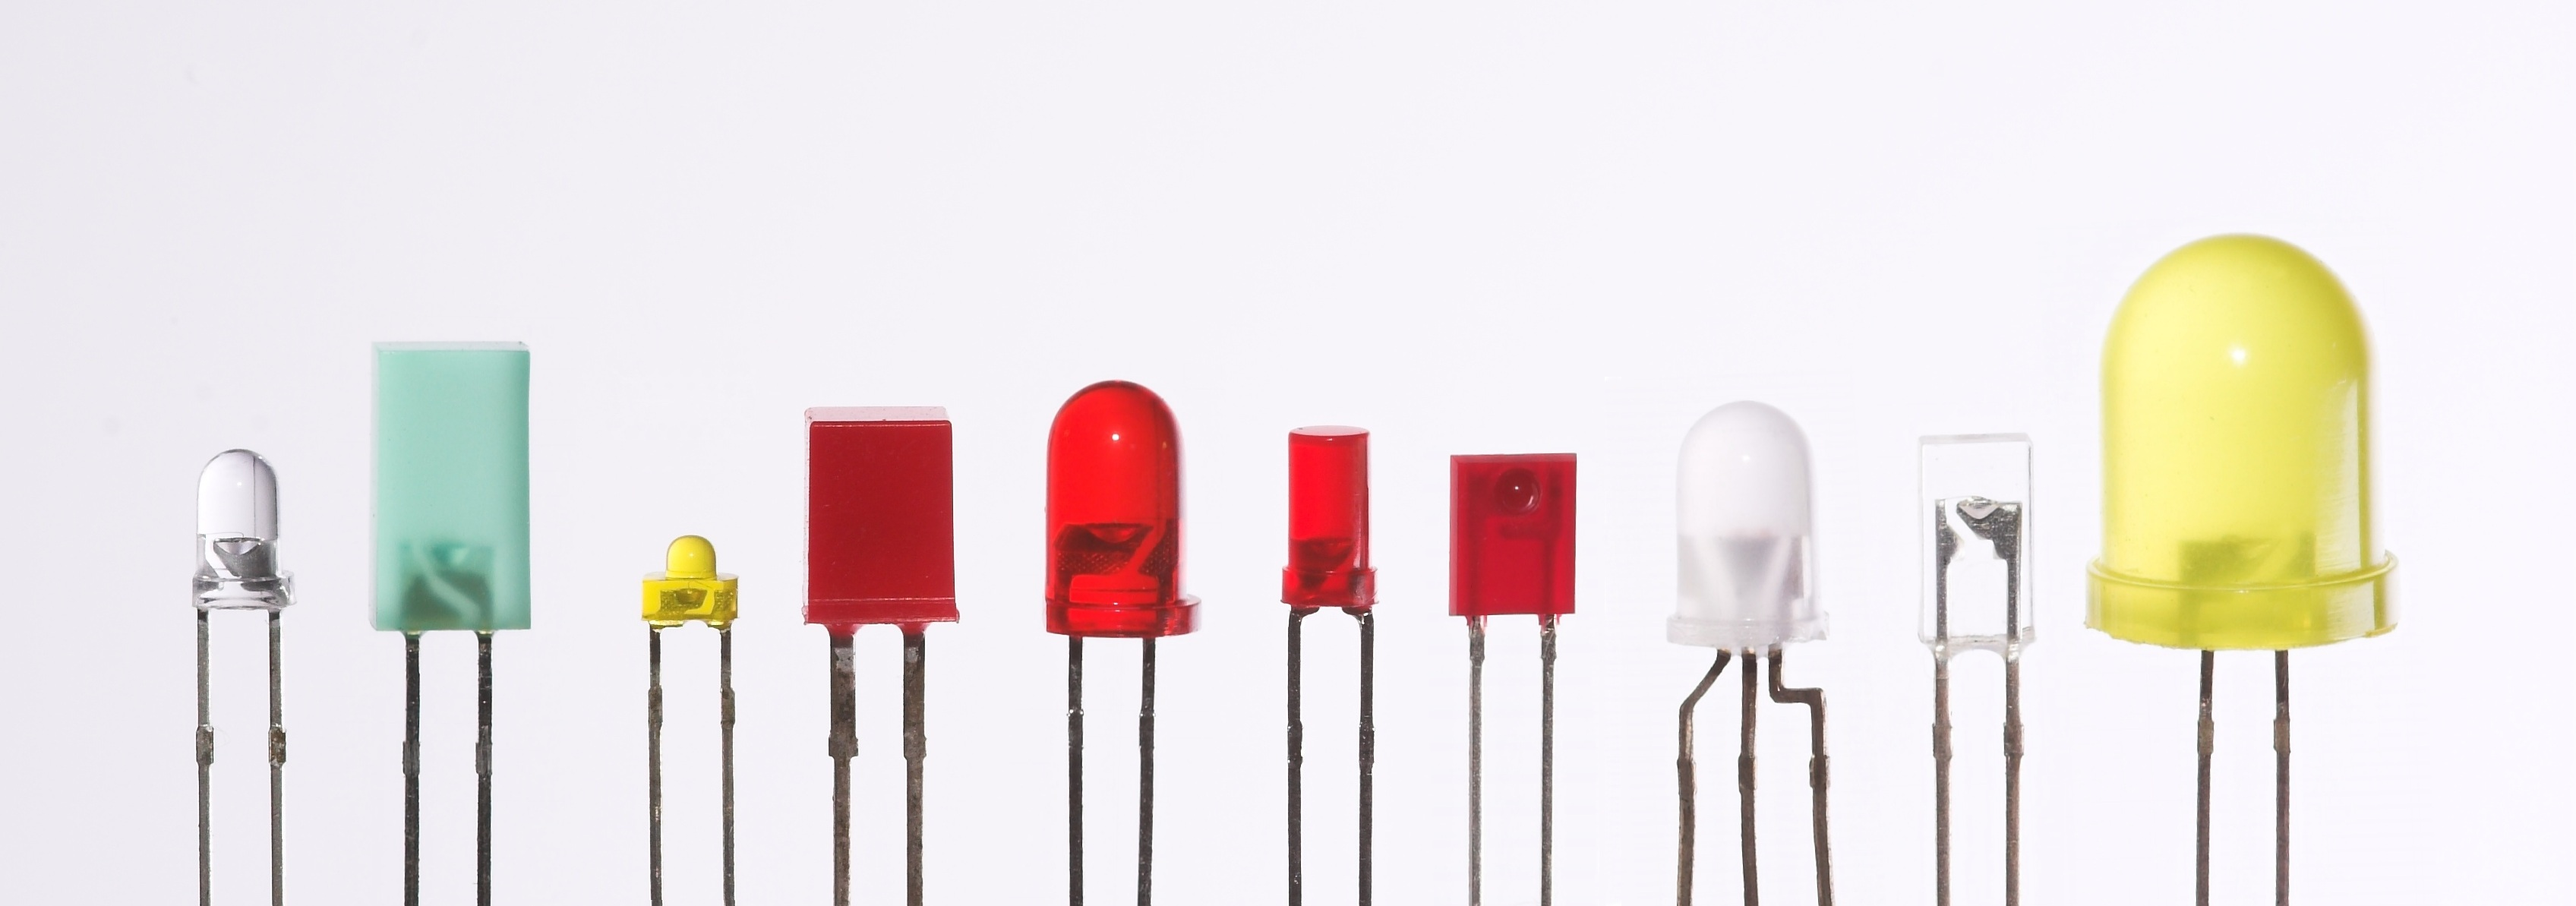
\includegraphics[width=\textwidth]{images/LEDs.jpg}

  {\tiny By Afrank99 - Own work, CC BY-SA 2.0,
    \url{https://commons.wikimedia.org/w/index.php?curid=248198}}
\end{frame}

\begin{frame}
  \frametitle{Un semaforo}
  \begin{center}
    \includegraphics[height=0.6\textheight]{images/semaphore-manual.pdf}
  \end{center}
\end{frame}

\begin{frame}
  \frametitle{Laboratorio}
  \begin{center}
    \LARGE
    Facciamo funzionare il semaforo!
  \end{center}
\end{frame}

\section{Automazione}

\begin{frame}
  \frametitle{Come lo comando automaticamente?}
  \begin{itemize}
  \item Ruota meccanica
  \item Circuito elettronico
  \item Computer
  \end{itemize}
\end{frame}

\begin{frame}
  \frametitle{Che cosa è un computer?}
  \begin{center}
    \includegraphics[height=0.6\textheight]{images/computer-model.pdf}
  \end{center}
\end{frame}

\begin{frame}
  \frametitle{Ma... quale computer?}
  \begin{itemize}
  \item I personal computer hanno vari connettori per dispositivi elettronici
    \begin{itemize}
    \item USB
    \item HDMI, VGA, Display port
    \item Schede di memoria SD
    \item Cuffie e microfono
    \item \dots
    \end{itemize}
  \item Molto potenti e semplici da usare
  \item Ma nessuno di questi agisce come un semplice interruttore
  \end{itemize}
\end{frame}

\begin{frame}
  \frametitle{Raspberry Pi 3}
  \begin{columns}
    \column{0.3\textwidth}
    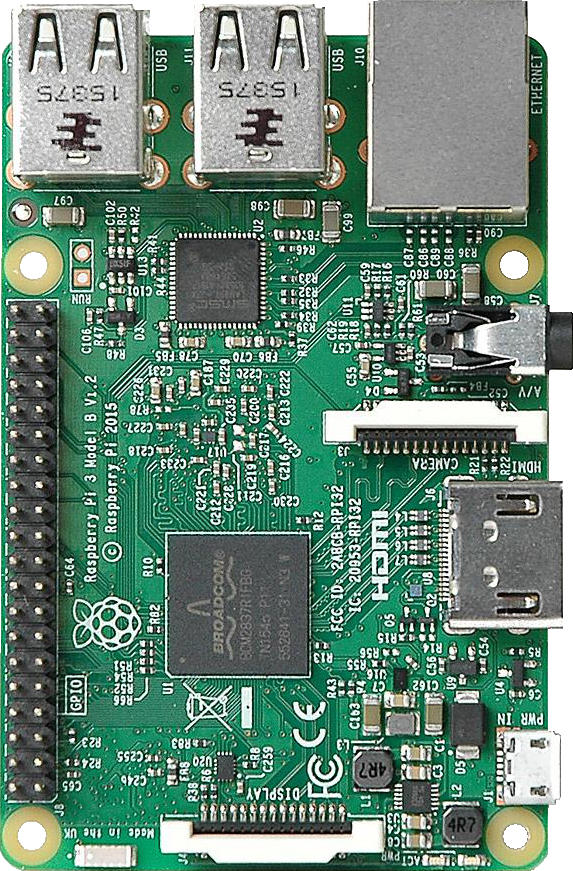
\includegraphics[width=\textwidth]{images/Raspberry_Pi_3_Model_B.jpg}
    \column{0.7\textwidth}
    \begin{itemize}
    \item 4-core ARM Cortex-A53 64 bit, 1.2 GHz
    \item 1 GB RAM
    \item Dispone di vari GPIO
      \begin{itemize}
      \item Contatti elettrici utilzzabili come interruttori o come ingressi
      \end{itemize}
    \item {\tiny
      \url{https://www.raspberrypi.org/products/raspberry-pi-3-model-b/}
      \url{http://elinux.org/RPi_Low-level_peripherals}
      \url{https://commons.wikimedia.org/wiki/File:Raspberry_Pi_3_Model_B.png}
    }
    \end{itemize}
  \end{columns}
\end{frame}

\section{Un semplice semaforo con Scratch}

\begin{frame}
  \frametitle{Schema di collegamento}
  \begin{center}
    \includegraphics[height=0.9\textheight]{images/semaphore-gpio.pdf}
  \end{center}
\end{frame}

\begin{frame}
  \frametitle{Comandare i GPIO con Scratch}
  \begin{center}
    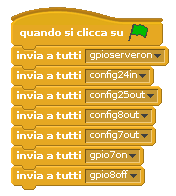
\includegraphics[height=0.8\textheight]{images/sketch-gpioserver.png}
  \end{center}
\end{frame}

\begin{frame}
  \frametitle{Laboratorio}
  \begin{columns}
    \column{0.6\textwidth}
    \begin{center}
      \LARGE Verde, giallo, rosso!
    \end{center}
    \column{0.4\textwidth}
    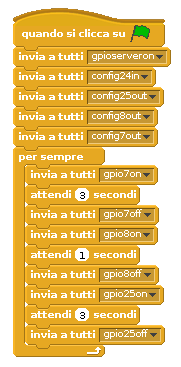
\includegraphics[height=0.8\textheight]{images/sketch-semaphore.png}
  \end{columns}
\end{frame}

\section{Un semaforo intelligente}

\begin{frame}
  \frametitle{Schema di collegamento}
  \begin{center}
    \includegraphics[height=0.9\textheight]{images/semaphore-gpio-pir.pdf}
  \end{center}
\end{frame}

\begin{frame}
  \frametitle{Leggere i GPIO con Scratch}
  \begin{center}
    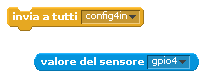
\includegraphics[height=0.25\textheight]{images/sketch-gpioserver2.png}
  \end{center}
\end{frame}

\begin{frame}
\frametitle{Laboratorio}
  \begin{center}
    \LARGE
    Semaforo intelligente
  \end{center}
\end{frame}

\section{E poi?}

\begin{frame}
  \frametitle{E poi?}
  \begin{itemize}
  \item Evoluzione di questo progetto
    \begin{itemize}
    \item Chiamata pedonale
    \item Lampeggiamento notturno
    \item Raccolta di statistiche sul traffico
    \end{itemize}
  \item Verso l'elettronica
    \begin{itemize}
    \item Arduino
    \item Progettazione hardware
    \end{itemize}
  \item Verso l'informatica
    \begin{itemize}
    \item Programmazione
    \item Amministrazione di server
    \end{itemize}
  \item Utilizzo del computer
  \end{itemize}
\end{frame}

\begin{frame}
  \frametitle{Fine}

  \begin{center}
    {\Huge Domande?}

    \vspace{0.1\textheight}

    \href{mailto:luca@lucaceresoli.net}{luca@lucaceresoli.net}\\
    \url{http://lucaceresoli.net}
  \end{center}
\end{frame}

\begin{frame}
  \frametitle{CC BY-SA}
  \begin{center}
    \textcopyright{} Copyright 2016, Luca Ceresoli\\

    \vspace{0.05\textheight}

    \small
    Materiale rilasciato sotto licenza\\
    Creative Commons Attribution - Share Alike 3.0 \\
    \url{https://creativecommons.org/licenses/by-sa/3.0/} \\
  \end{center}
\end{frame}

\end{document}
